\documentclass{beamer}

\usetheme{Madrid}
\usecolortheme{default}
\setbeamertemplate{navigation symbols}{}

\title{CS Exebit 2026}
\subtitle{Lean for Verification}
\author{Pranav Ramesh}
\date{}

\usepackage{amsmath}
\usepackage{amssymb}
\usepackage{listings}
\usepackage{xcolor}
\usepackage{graphicx}

\lstset{
  language=Java,
  basicstyle=\ttfamily\small,
  keywordstyle=\color{blue},
  commentstyle=\color{gray},
  stringstyle=\color{red},
  breaklines=true,
  showstringspaces=false
}

\begin{document}

\begin{frame}[fragile]
  \vspace*{\fill}
  \centering
  
\includegraphics[height=0.3\textheight]{logo.png}\\
  \vspace{0.5cm}
  {\Huge\textbf{\inserttitle}}\\
  \vspace{0.3cm}
  {\Large\textit{\insertsubtitle}}\\
  \vspace{0.5cm}
  {\large\insertauthor}\\
  \vspace*{\fill}
\end{frame}

% Section: Preface
\section{Preface}

\begin{frame}
  \frametitle{Proof Assistants}
  
  What are proof assistants (interactive theorem provers)?
  
  \begin{itemize}
    \item Check and help develop formal proofs
    \item Can prove big theorems, not just logic puzzles
    \item Can be tedious to use
    \item Highly addictive (think video games!)
  \end{itemize}
\end{frame}

\begin{frame}
  \frametitle{Classification by Logical Foundations}
  
  \begin{columns}
    \column{0.5\textwidth}
    \textbf{Set Theory:}
    \begin{itemize}
      \item Isabelle/ZF
      \item Metamath
      \item Mizar
    \end{itemize}
    
    \column{0.5\textwidth}
    \textbf{Simple Type Theory:}
    \begin{itemize}
      \item HOL4
      \item HOL Light
      \item Isabelle/HOL
      \item PVS
    \end{itemize}
  \end{columns}
  
  \vspace{0.5cm}
  
  \textbf{Dependent Type Theory:}
  \begin{itemize}
    \item Agda
    \item \textbf{Lean} ← We focus here
    \item Matita
    \item Rocq
  \end{itemize}
\end{frame}

\begin{frame}
  \frametitle{Success Stories in Formal Verification}
  
  \textbf{Mathematics:}
  \begin{itemize}
    \item The four-color theorem
    \item The Kepler conjecture
    \item The definition of perfectoid spaces
  \end{itemize}
  
  \vspace{0.3cm}
  
  \textbf{Computer Science:}
  \begin{itemize}
    \item Hardware verification
    \item Operating systems
    \item Programming language theory
    \item Compilers
    \item Security
  \end{itemize}
\end{frame}

\begin{frame}
  \frametitle{What is Lean?}
  
  \begin{itemize}
    \item Proof assistant developed by Leonardo de Moura (AWS) since 2012
    \item Mathematical library \texttt{mathlib} developed by large community
    \item Community version of Lean 4
    \item Built on the \textbf{calculus of inductive constructions}
  \end{itemize}
  
  \vspace{0.3cm}
  
  \textbf{Key Features:}
  \begin{itemize}
    \item Highly expressive dependent type theory
    \item Extended with classical axioms and quotient types
    \item Modern metaprogramming framework
    \item Modern user interface
    \item Open source with active community
  \end{itemize}
\end{frame}


% Section: Types and Terms
\section{Types and Terms}

\begin{frame}
  \frametitle{A View of Lean}
  
  \begin{center}
    \Large
    Lean = Functional Programming + Logic
  \end{center}
  
  \vspace{0.5cm}
  
  Today's focus:
  \begin{itemize}
    \item Syntax of types and terms
    \item Basics of Functional Programming
    \item Proof Automation and metaprogramming
  \end{itemize}
\end{frame}

\begin{frame}
  \frametitle{Types}
  
  Types $\alpha$, $\tau$, $\nu$ can be:
  
  \begin{itemize}
    \item Type variables: $\alpha$
    \item Basic types: $T$
    \item Complex types: $T\,\sigma_1\,\ldots\,\sigma_N$
  \end{itemize}
  
  \vspace{0.3cm}
  
  \textbf{Function Types:}
  \begin{itemize}
    \item Some type constructors written infix (e.g., →)
    \item Right-associative: $\sigma_1 \to \sigma_2 \to \sigma_3 \to \tau = \sigma_1 \to (\sigma_2 \to (\sigma_3 \to \tau))$
  \end{itemize}
  
  \vspace{0.3cm}
  
  \textbf{Polymorphism:}
  \begin{itemize}
    \item Type variables must be bound using $\forall$
    \item Example: $\forall \alpha,\, \alpha \to \alpha$
  \end{itemize}
\end{frame}

\begin{frame}
  \frametitle{Terms and Applications}
  
  Terms $t$, $u$:
  
  \begin{itemize}
    \item Constants $c$
    \item Variables $x$
    \item Applications $t\,u$
    \item Anonymous functions $\lambda x \mapsto t$
  \end{itemize}
  
  \vspace{0.3cm}
  
  \textbf{Currying:}
  Functions can be:
  \begin{itemize}
    \item Fully applied: $f\,x\,y\,z$
    \item Partially applied: $f\,x\,y$ or $f\,x$
    \item Unapplied: $f$
  \end{itemize}
  
  \vspace{0.3cm}
  
  Application is left-associative: $f\,x\,y\,z = ((f\,x)\,y)\,z$
\end{frame}

\begin{frame}
  \frametitle{Type Checking and Inference}
  
  \textbf{Key Facts:}
  \begin{itemize}
    \item Both type checking and type inference are decidable
    \item This property is lost with overloading or subtyping
  \end{itemize}
  
  \vspace{0.3cm}
  
  \textbf{Type Judgment:} $\Gamma \vdash t : \sigma$
  
  Means: $t$ has type $\sigma$ in local context $\Gamma$
\end{frame}

\begin{frame}
  \frametitle{Typing Rules}
  
  \textbf{Constant:}
  $$\frac{}{\Gamma \vdash c : \sigma} \quad \text{(if $c$ declared with type $\sigma$)}$$
  
  \textbf{Variable:}
  $$\frac{}{\Gamma \vdash x : \sigma} \quad \text{(if $x : \sigma$ in $\Gamma$)}$$
  
  \textbf{Application:}
  $$\frac{\Gamma \vdash t : \sigma \to \tau \quad \Gamma \vdash u : \sigma}{\Gamma \vdash t\,u : \tau}$$
  
  \textbf{Abstraction:}

  $$\frac{\Gamma, x : \sigma \vdash t : \tau}{\Gamma \vdash (\lambda x : \sigma \mapsto t) : \sigma \to \tau}$$
\end{frame}


% Section: Transition Systems
\section{Transition Systems}


\begin{frame}[fragile]
  \frametitle{Transition Systems - Page 2}
  \centering
  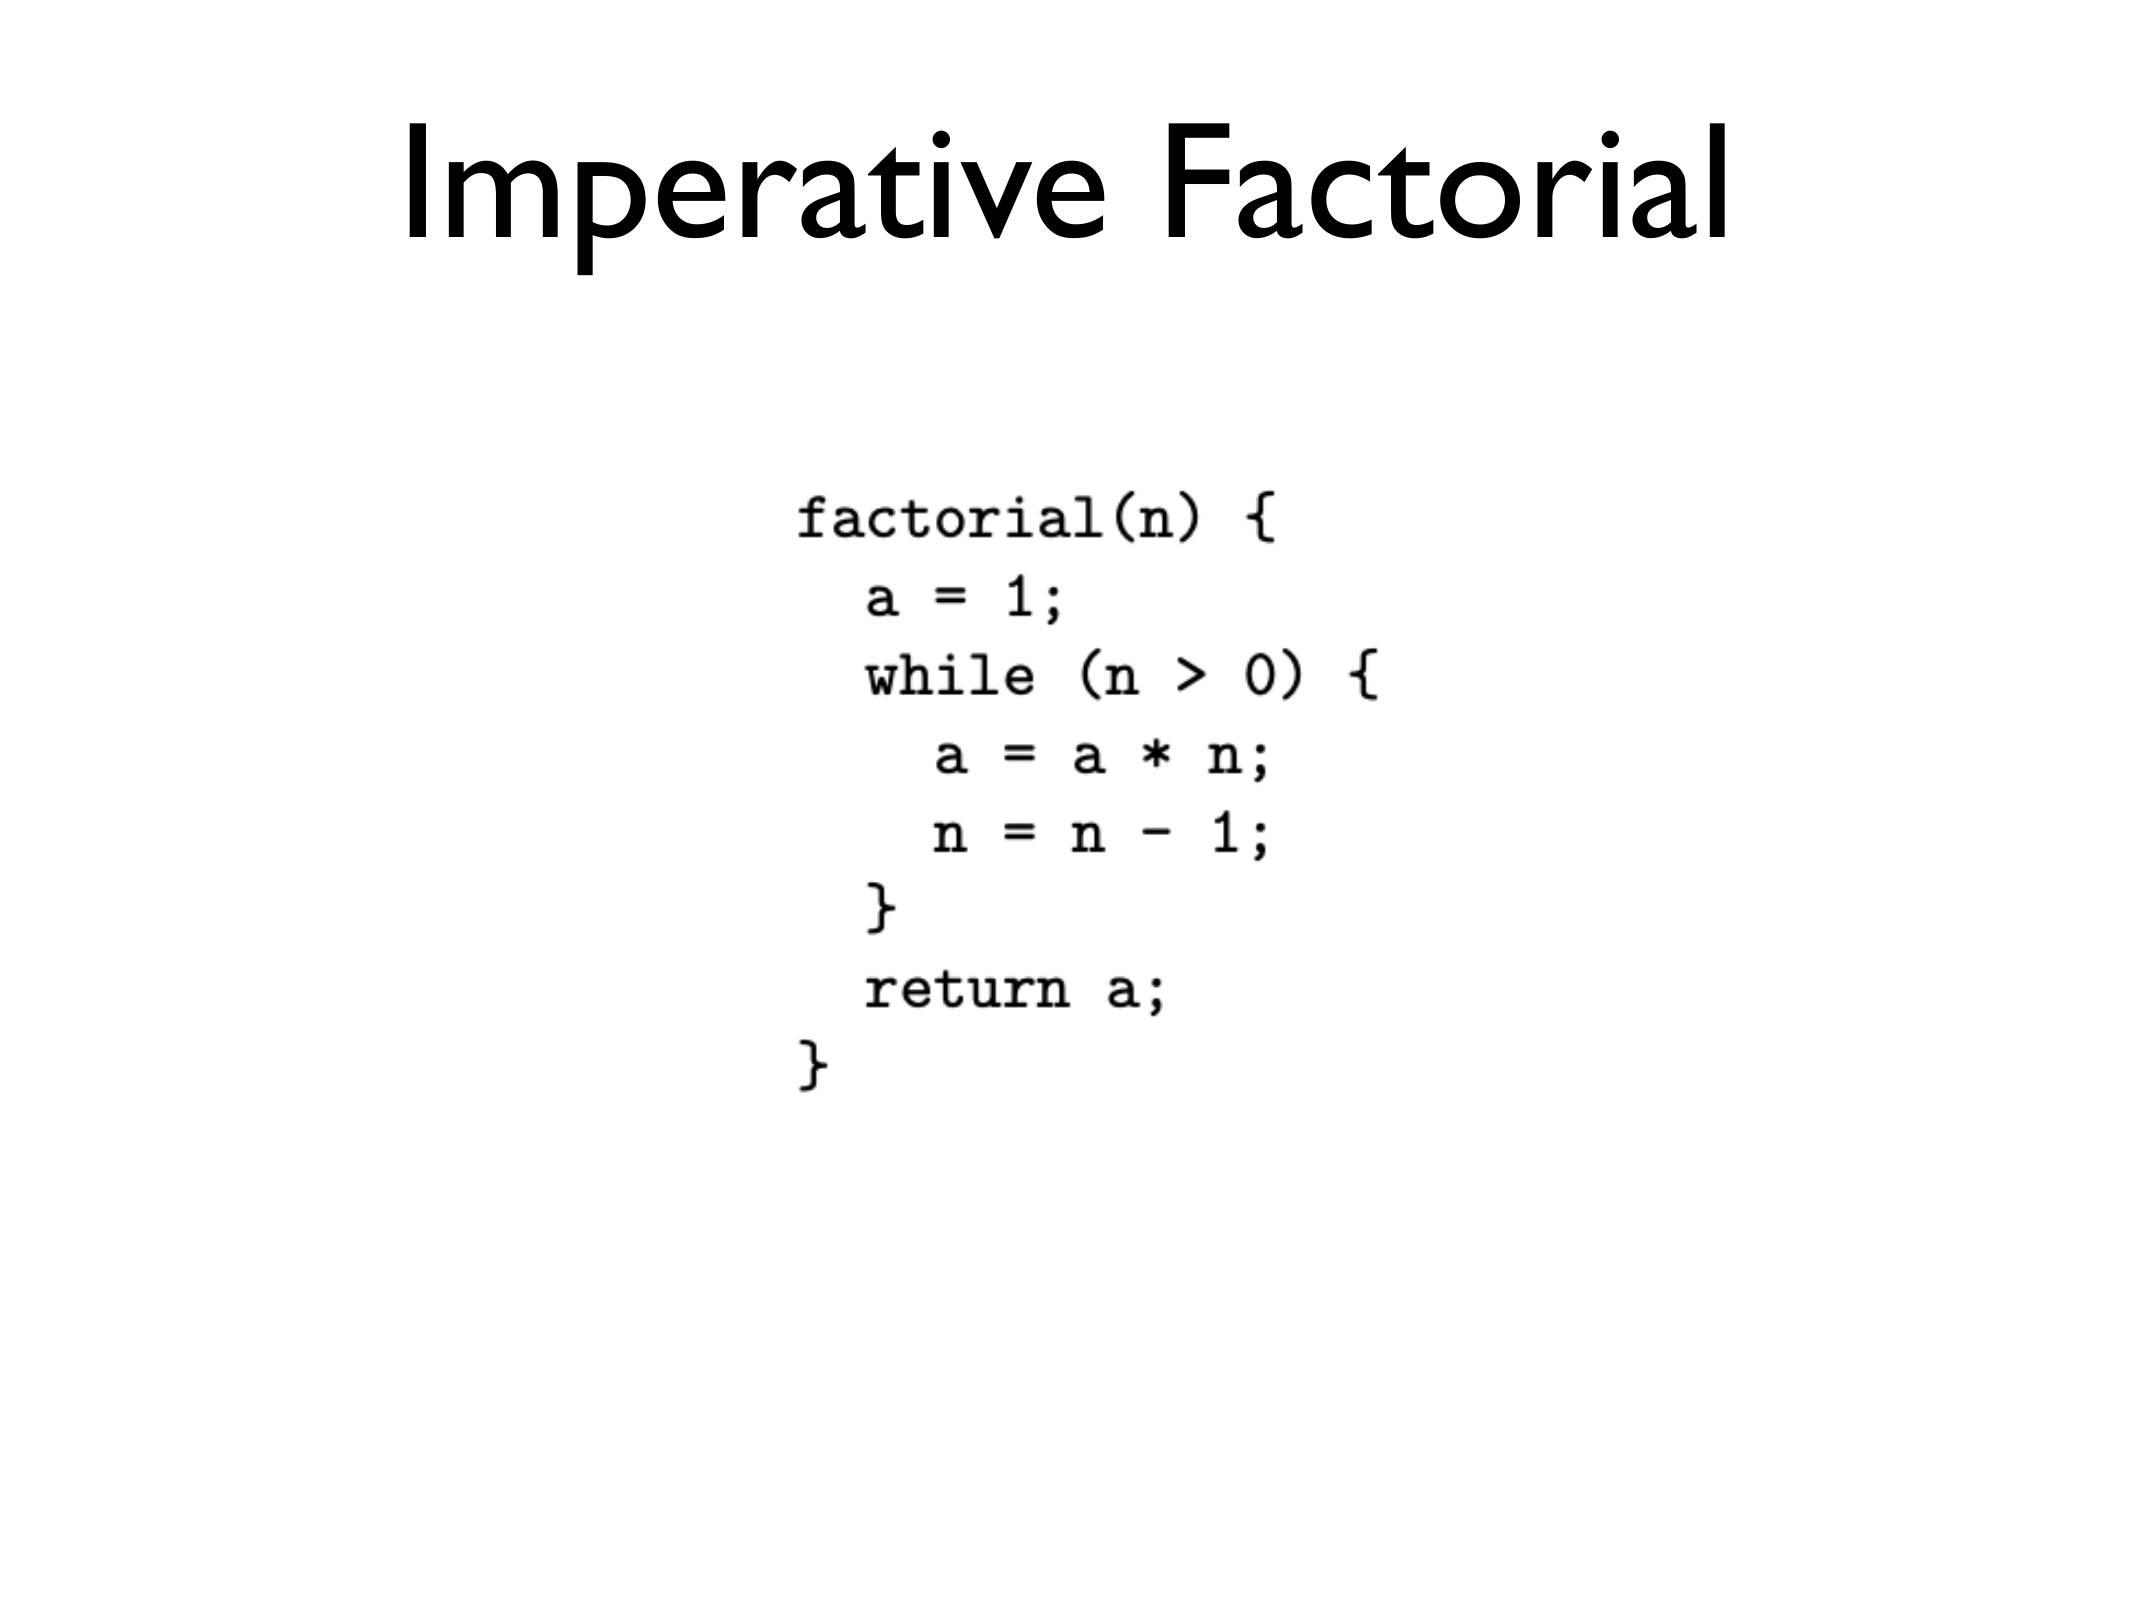
\includegraphics[width=\textwidth,height=0.85\textheight,keepaspectratio]{transition_systems-2.png}
\end{frame}

\begin{frame}[fragile]
  \frametitle{Transition Systems - Page 3}
  \centering
  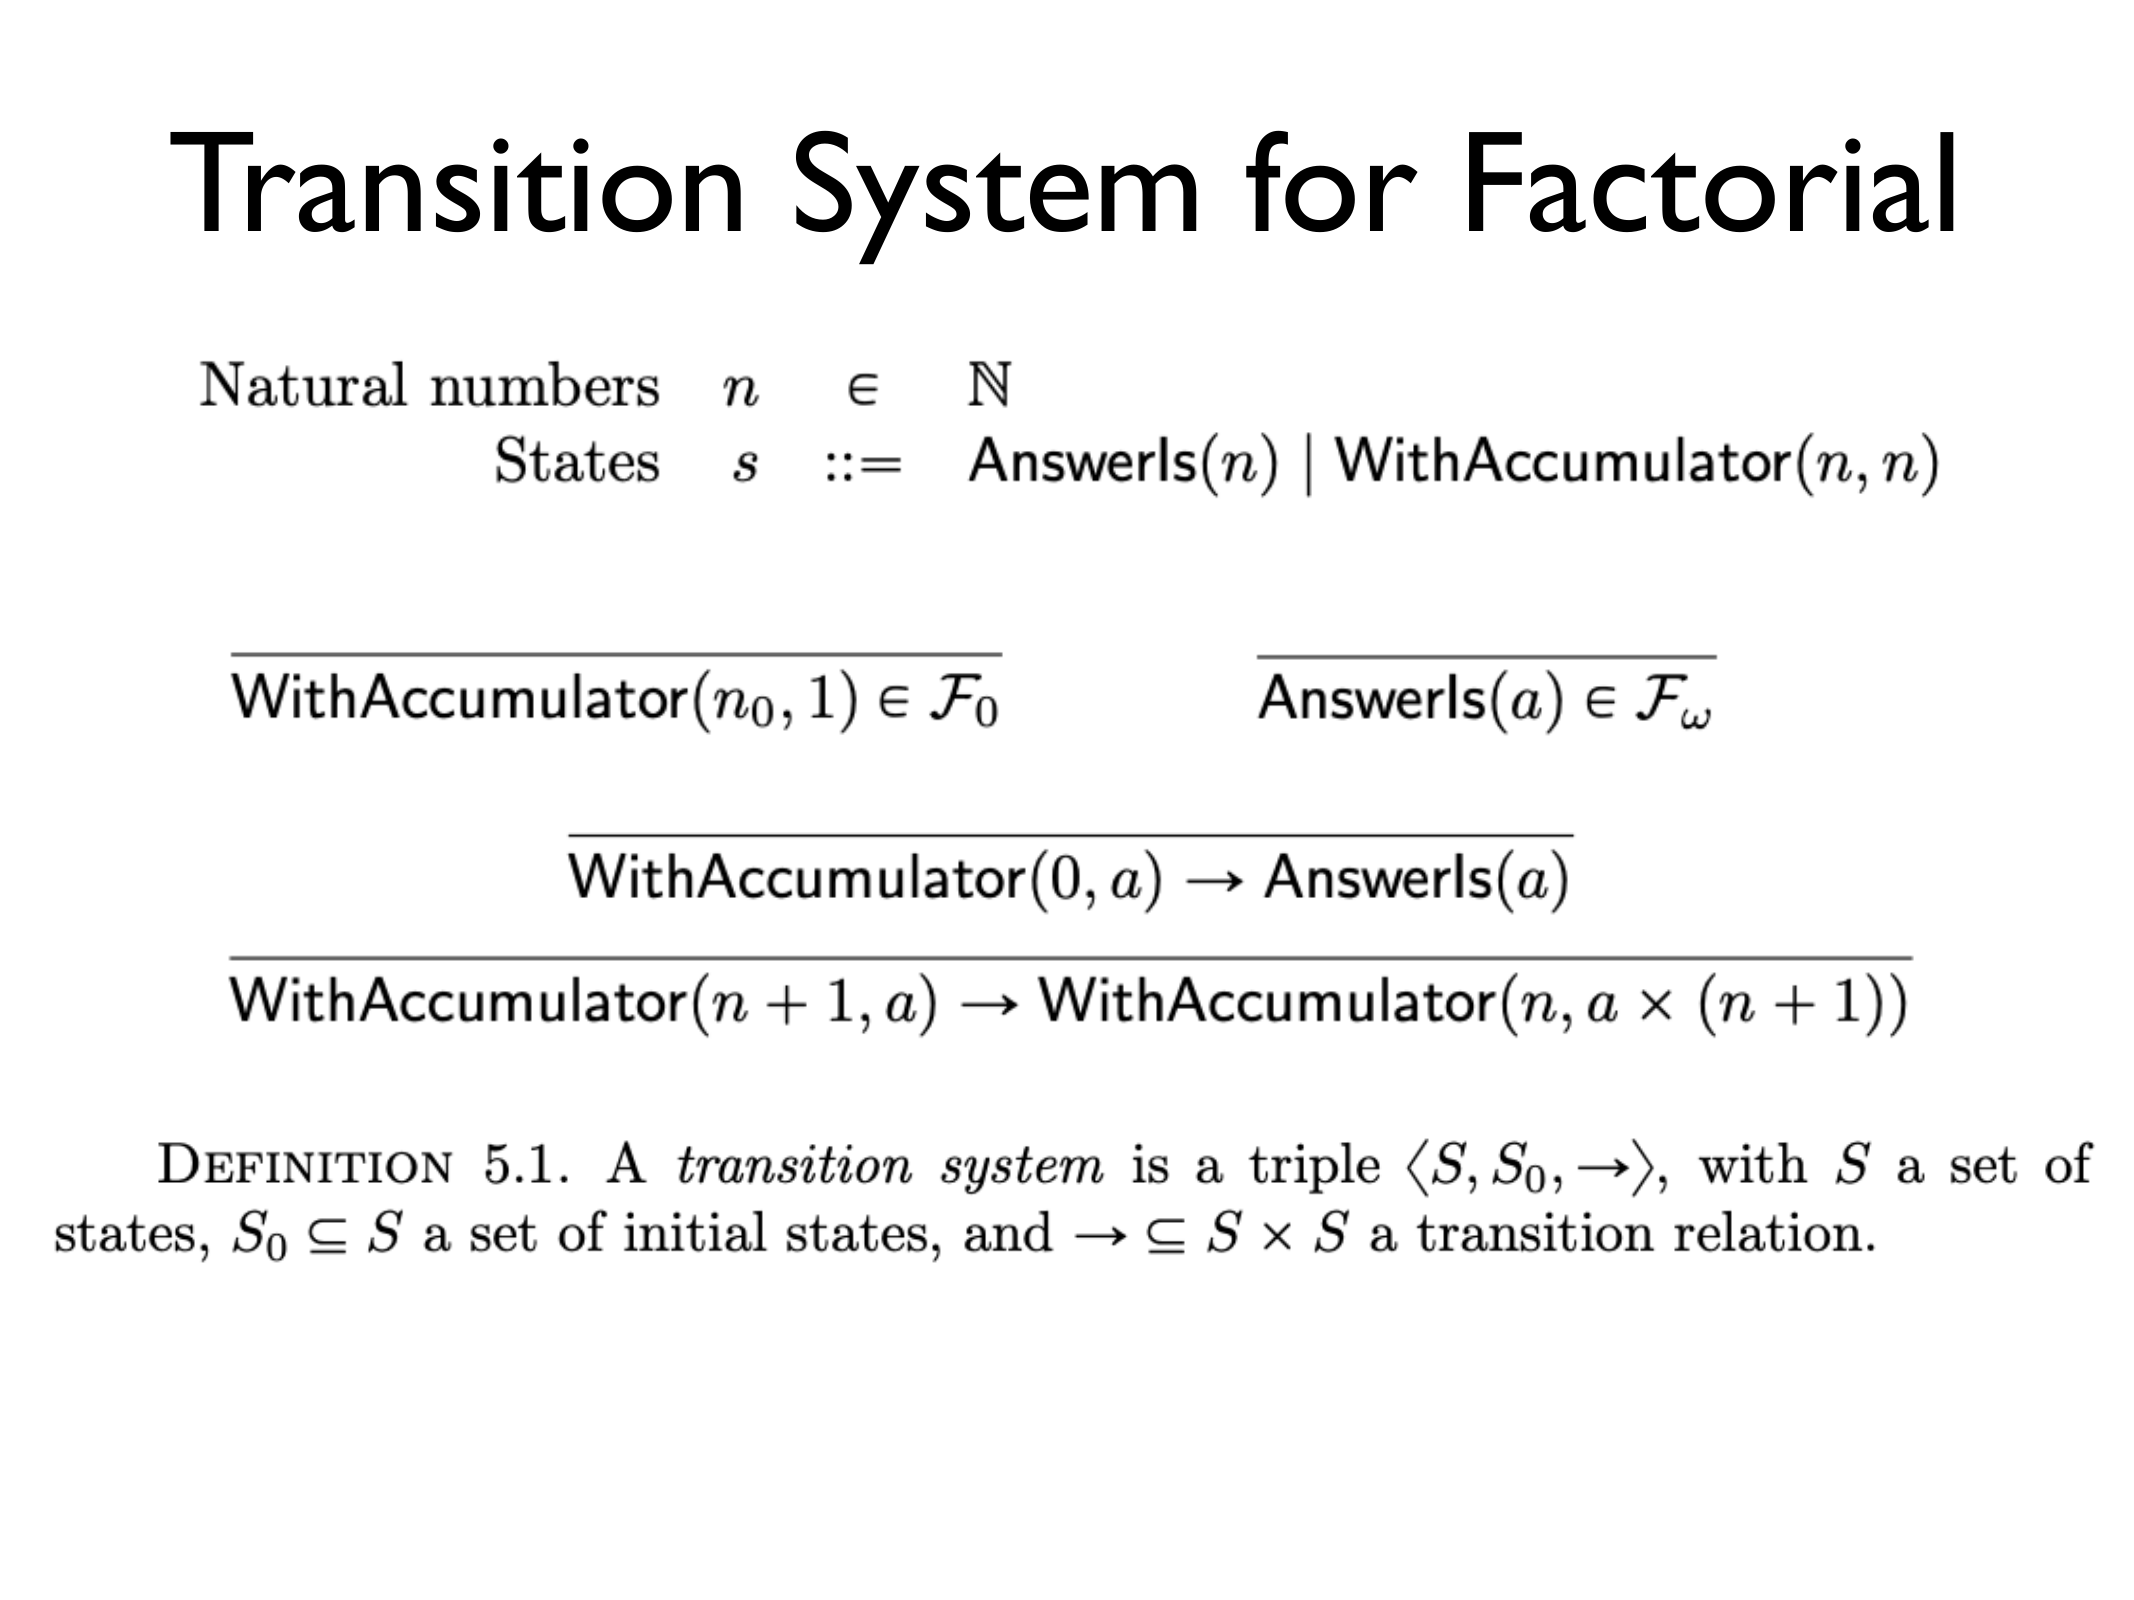
\includegraphics[width=\textwidth,height=0.85\textheight,keepaspectratio]{transition_systems-3.png}
\end{frame}

\begin{frame}[fragile]
  \frametitle{Transition Systems - Page 4}
  \centering
  
\includegraphics[width=\textwidth,height=0.85\textheight,keepaspectratio]{transition_systems-4.png}
\end{frame}

\begin{frame}[fragile]
  \frametitle{Transition Systems - Page 5}
  \centering
  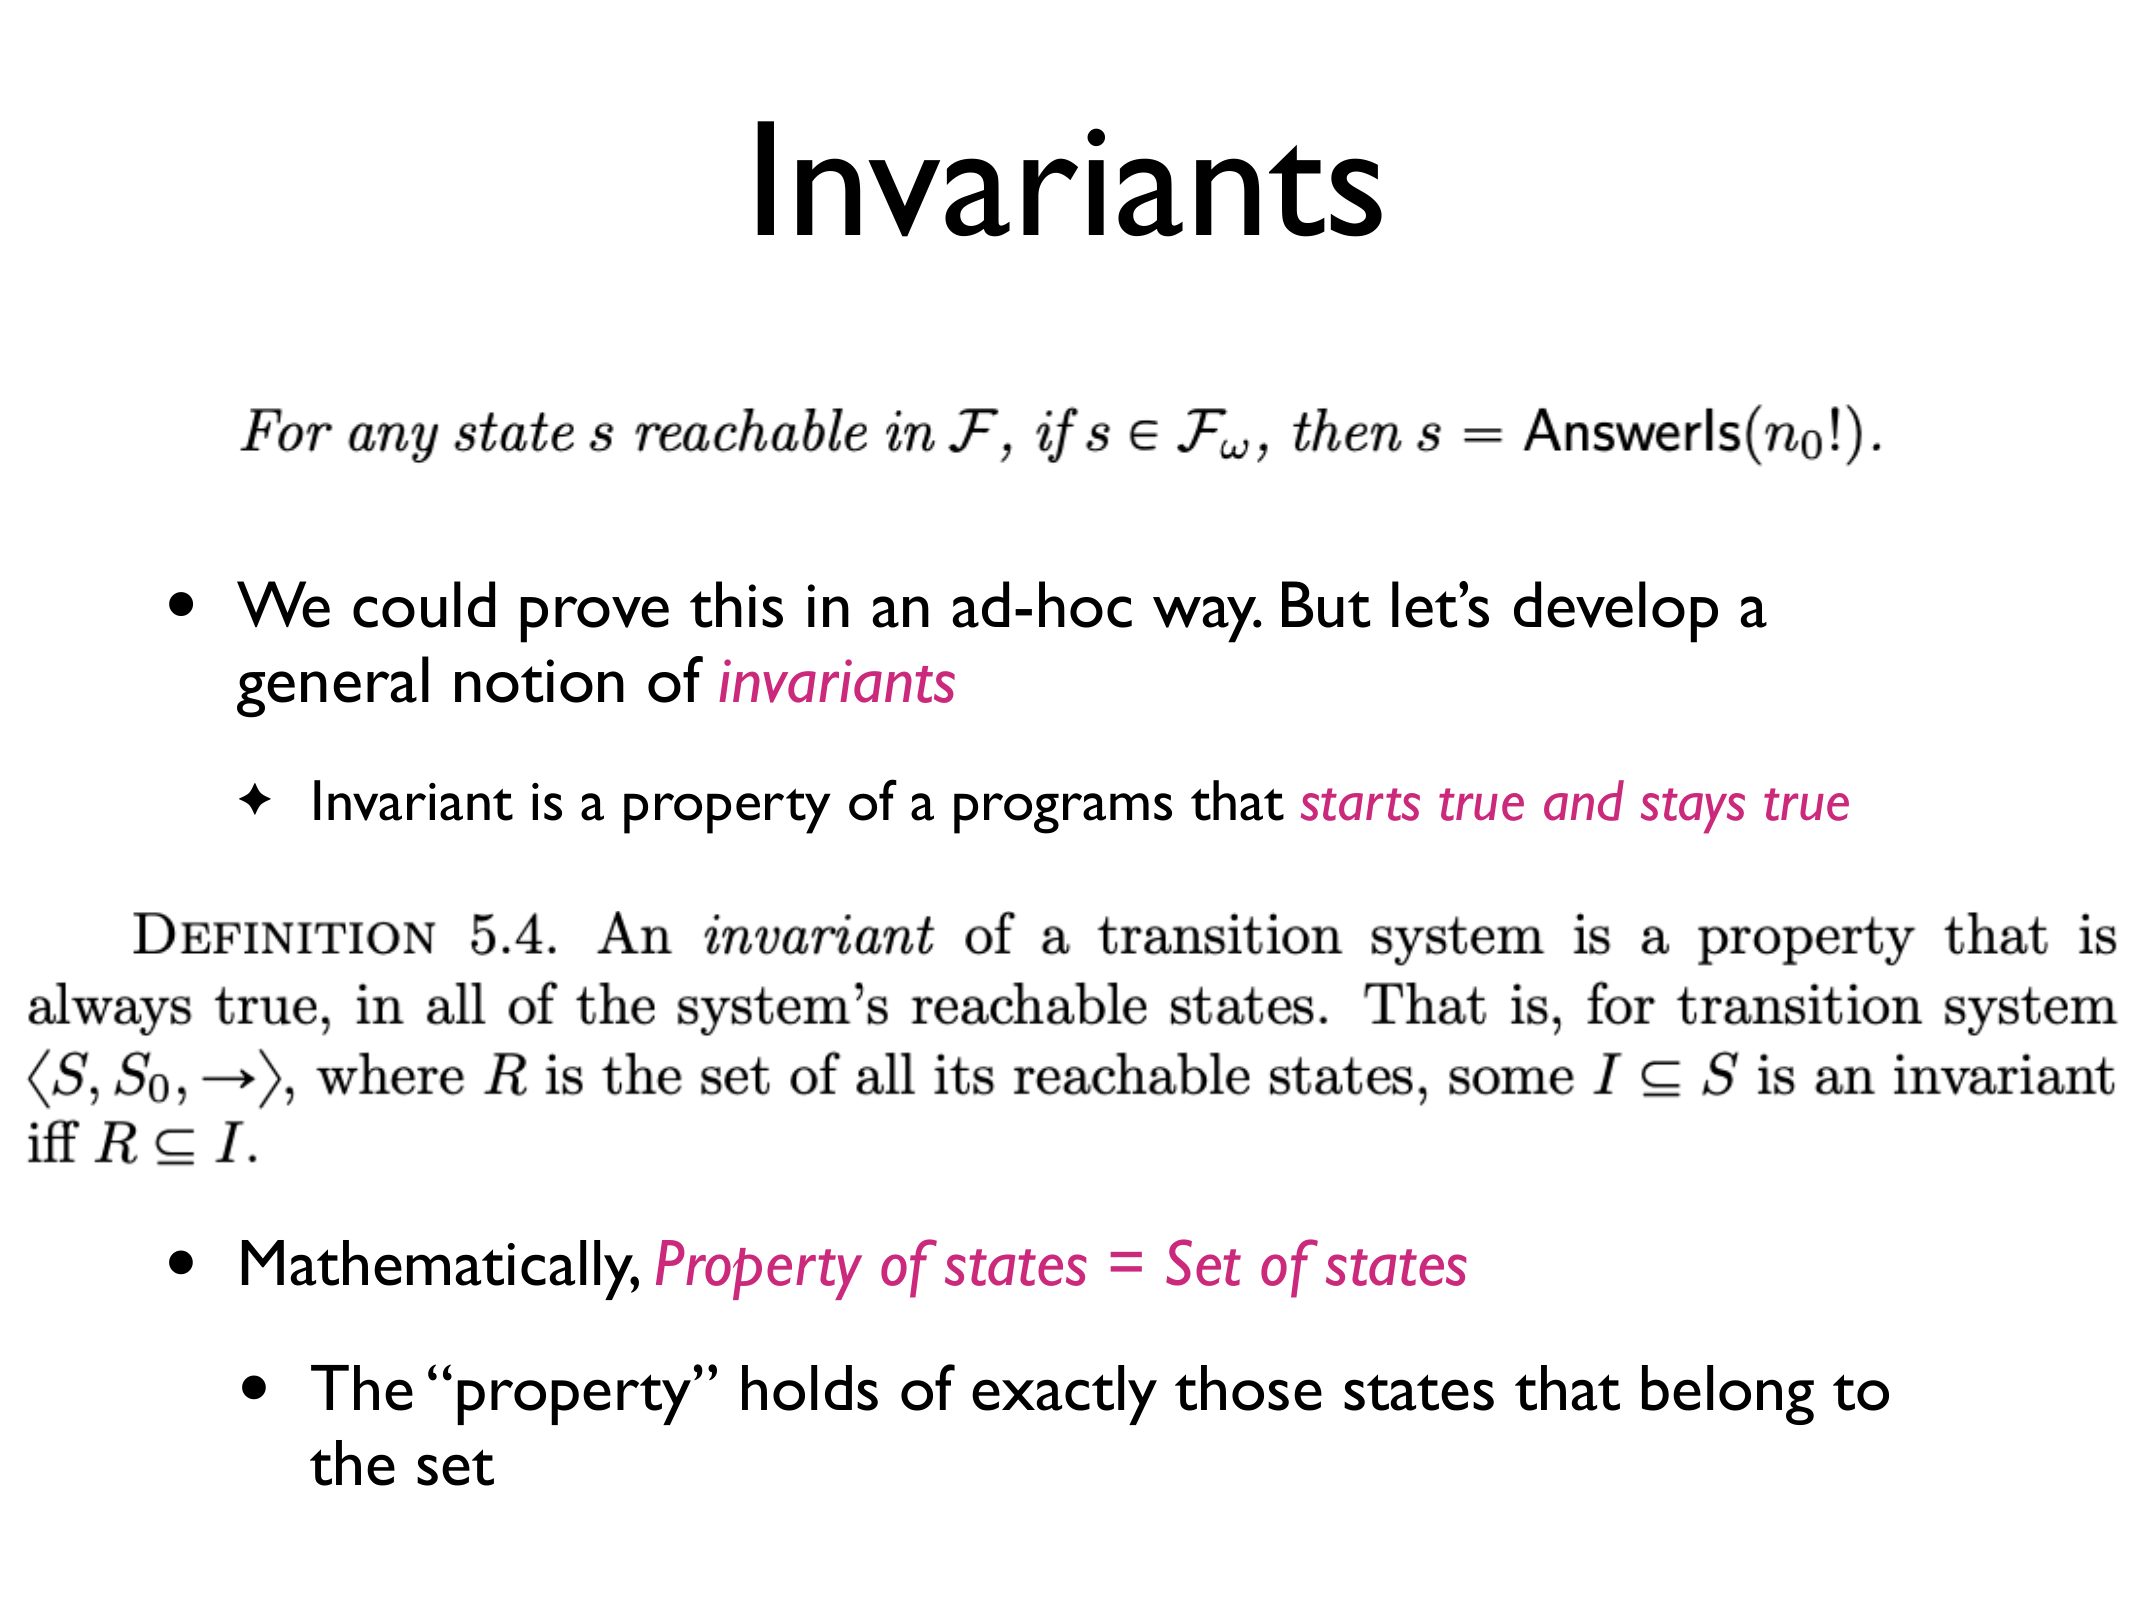
\includegraphics[width=\textwidth,height=0.85\textheight,keepaspectratio]{transition_systems-5.png}
\end{frame}

\end{document}
